\documentclass[a4paper]{report}
\usepackage[utf8]{inputenc}
\usepackage[portuguese]{babel}
\usepackage{hyperref}
\usepackage{a4wide}
\hypersetup{pdftitle={AP - Rooms},
pdfauthor={João Teixeira, José Ferreira},
colorlinks=true,
urlcolor=blue,
linkcolor=black}
\usepackage{subcaption}
\usepackage{listings}
\usepackage{booktabs}
\usepackage{multirow}
\usepackage{appendix}
\usepackage{tikz}
\usepackage{authblk}
\usepackage{bashful}
\usepackage{verbatim}
\usepackage{amssymb}
\usepackage{multirow}
\usepackage{mwe}
\usepackage[parfill]{parskip}
\usetikzlibrary{positioning,automata,decorations.markings}
\AfterEndEnvironment{figure}{\noindent\ignorespaces}
\AfterEndEnvironment{table}{\noindent\ignorespaces}

\begin{document}

\title{Algoritmos Paralelos\\Room Assignment Problem}
\author{João Teixeira (A85504) \and José Filipe Ferreira (A83683)}
\date{\today}

\begin{center}
    \begin{minipage}{0.75\linewidth}
        \centering
        
\includegraphics[width=0.4\textwidth]{images/eng.jpeg}\par\vspace{1cm}
        \vspace{1.5cm}
        \href{https://www.uminho.pt/PT}
        {\color{black}{\scshape\LARGE Universidade do Minho}} \par
        \vspace{1cm}
        \href{https://www.di.uminho.pt/}
        {\color{black}{\scshape\Large Departamento de Informática}} \par
        \vspace{1.5cm}
        \maketitle
    \end{minipage}
\end{center}

\tableofcontents

\pagebreak

\chapter{Introdução}
O \textit{room assignment problem} consiste em distribuir n pessoas por n/2
salas de forma a minimizar os maus relacionamentos entre os habitantes de cada
sala. A única maneira de obter o melhor resultado para este algoritmo consiste
em testar todas as possibilidades, calcular um valor para cada um com recurso a
uma função objetivo e procurar o menor entre eles. Resolver este problema com
forca bruta resulta numa complexidade de O(n!) fazendo com que o tempo da
computação aumente de forma extremamente rápida.

Para contornar este problema é possível recorrer a métodos que, apesar de não
calcularem o melhor resultado possível, conseguem calcular uma aproximação do
resultado final. Para tal pode-se desenvolver algoritmos determinísticos
(\textit{greedy search}) e algoritmos não determinísticos.

Um problema NP, ou seja, um problema polinomial em tempo não determinístico é
uma classe utilizada para classificar um sub conjunto de problemas de decisão.
Estes problemas são caracterizados por ser possível calcular um resultado de
forma não determinística em tempo polinomial. A solução NP foi desenvolvida
fazendo uso do método de Monte-Carlo com e sem \textit{annealing}.

Ao longo deste relatório iremos descrever em mais detalhe como desenvolvemos
estes algoritmos e comparar os resultados obtidos entre eles.

\chapter{Soluções desenvolvidas}


Internamente os dados são representados da seguinte forma:
\begin{itemize}
    \item Cada pessoa tem um id associado de 0 ate n-1;
    \item O relacionamento entre a pessoa i e a pessoa j é dado pelo valor
        D(i,j) contido numa matriz simétrica D com valores entre 1 e 10;
    \item As salas são uma matriz n/2 por 2 em que cada sala é uma coluna;
\end{itemize}

Dentro de cada teste, cada algoritmo determinístico foi executado uma vez e cada
algoritmo não determinístico foi executado mil vezes fazendo uso sempre da mesma
matriz de relacionamentos populada de forma aleatória no inicio do teste.

\section{Greedy Search}

Este método consiste em percorrer todas as salas uma a uma. Para cada sala
procura-se quais são as pessoas que se dão melhor para as quais ainda não foi
atribuída uma sala e coloca se nessa mesma sala. Desta forma o algoritmo é
determinístico e polinomial.

A complexidade de percorrer cada sala é O(n/2), para procurar qual é o par que
vai ocupar cada sala a complexidade é O(n²/2 - n). Multiplicando uma pela outra
obtemos que a complexidade do algoritmo é O(n³). Resultando numa complexidade
muito menor do que a complexidade do algoritmo de \textit{brute froce} para um n
suficientemente grande.

\section{Monte-Carlo}

Por contraste com o método de \textit{greedy search}, o método de Monte-Carlo é
não determinístico.

No inicio do calculo, preenche-se as salas com uma permutação aleatória de
pessoas de forma a obter um estado inicial. Em seguida calcula-se o custo desse
estado inicial.

Para melhorar o resultado do estado inicial cria-se um loop que corre um
conjunto de passos. Primeiro calcula-se duas salas consecutivas e compara-se a
diferença de custo se os membros dessas salas fossem trocados. Caso o custo
fique mais baixo a troca é efetivada e o custo final atualizado. Caso ocorram
maxi loops ao sem ser feita nenhuma troca o algoritmo termina.

\section{Monte-Carlo com Annealing}

O metodo de Monte-Carlo com \textit{Annealing} é muito semelhante ao método de
Monte-Carlo sem \textit{annealing}. Primeiro é introduzido o conceito de
temperatura. A temperatura começa a 1. E em cada ciclo a temperatura decai
seguindo a formula T = T * Tdecay. Assim que a temperatura atinge um Tmin as
iterações acabam. Aquando de decidir se a ordem das salas e trocada ou não
existe uma clausula extra definida por exp(-delta/temperatura) <= rand.

\chapter{Analise de Resultados}

Para representar os resultados obtidos decidimos utilizar um gráfico de caixa,
de forma a mostrar a concentração dos resultados, bem como os seus extremantes.

\begin{figure}[h]
\centering
\begin{minipage}{.5\textwidth}
  \centering
  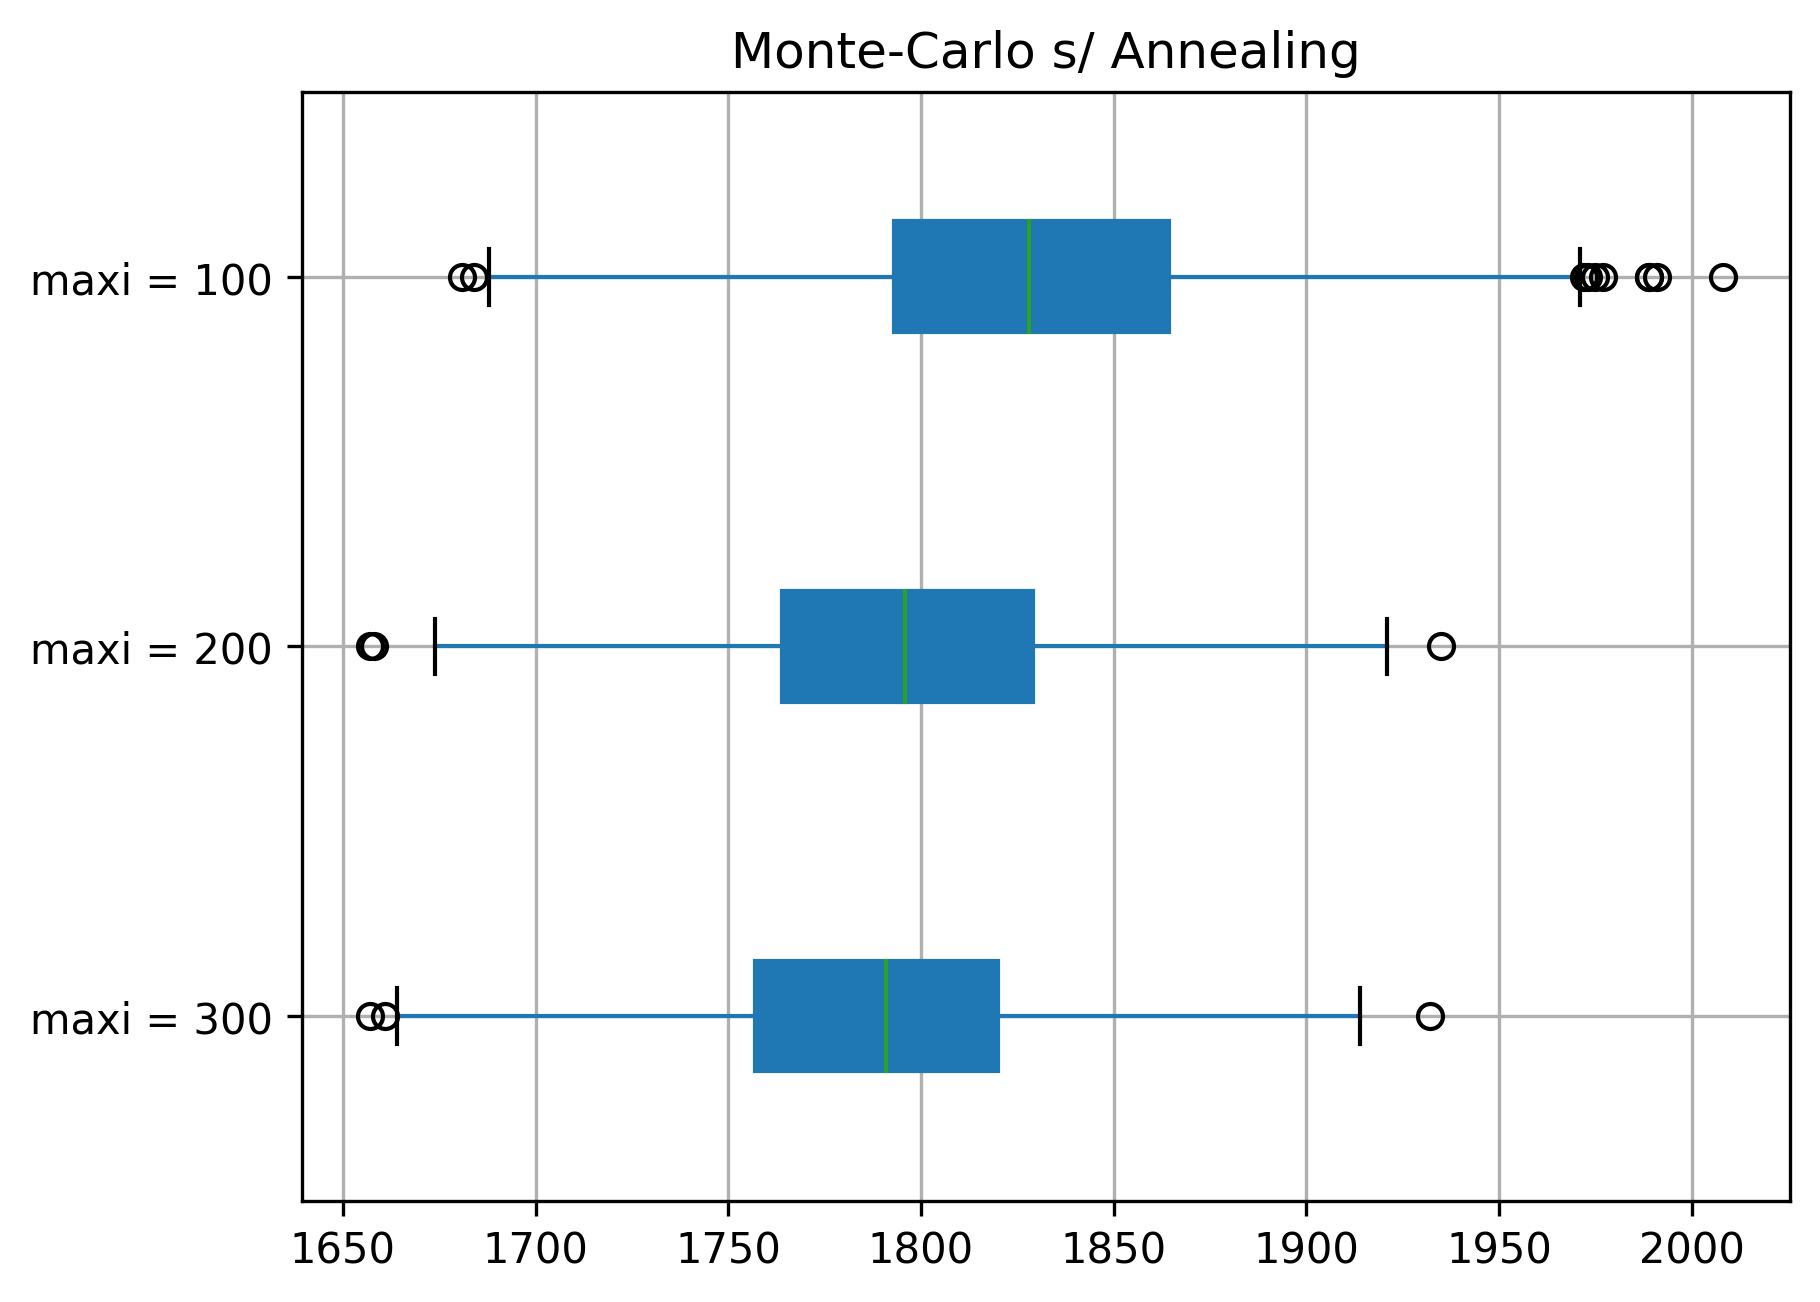
\includegraphics[width=.95\linewidth]{images/graph_comp_maxi_mc.png}
\end{minipage}%
\begin{minipage}{.5\textwidth}
  \centering
  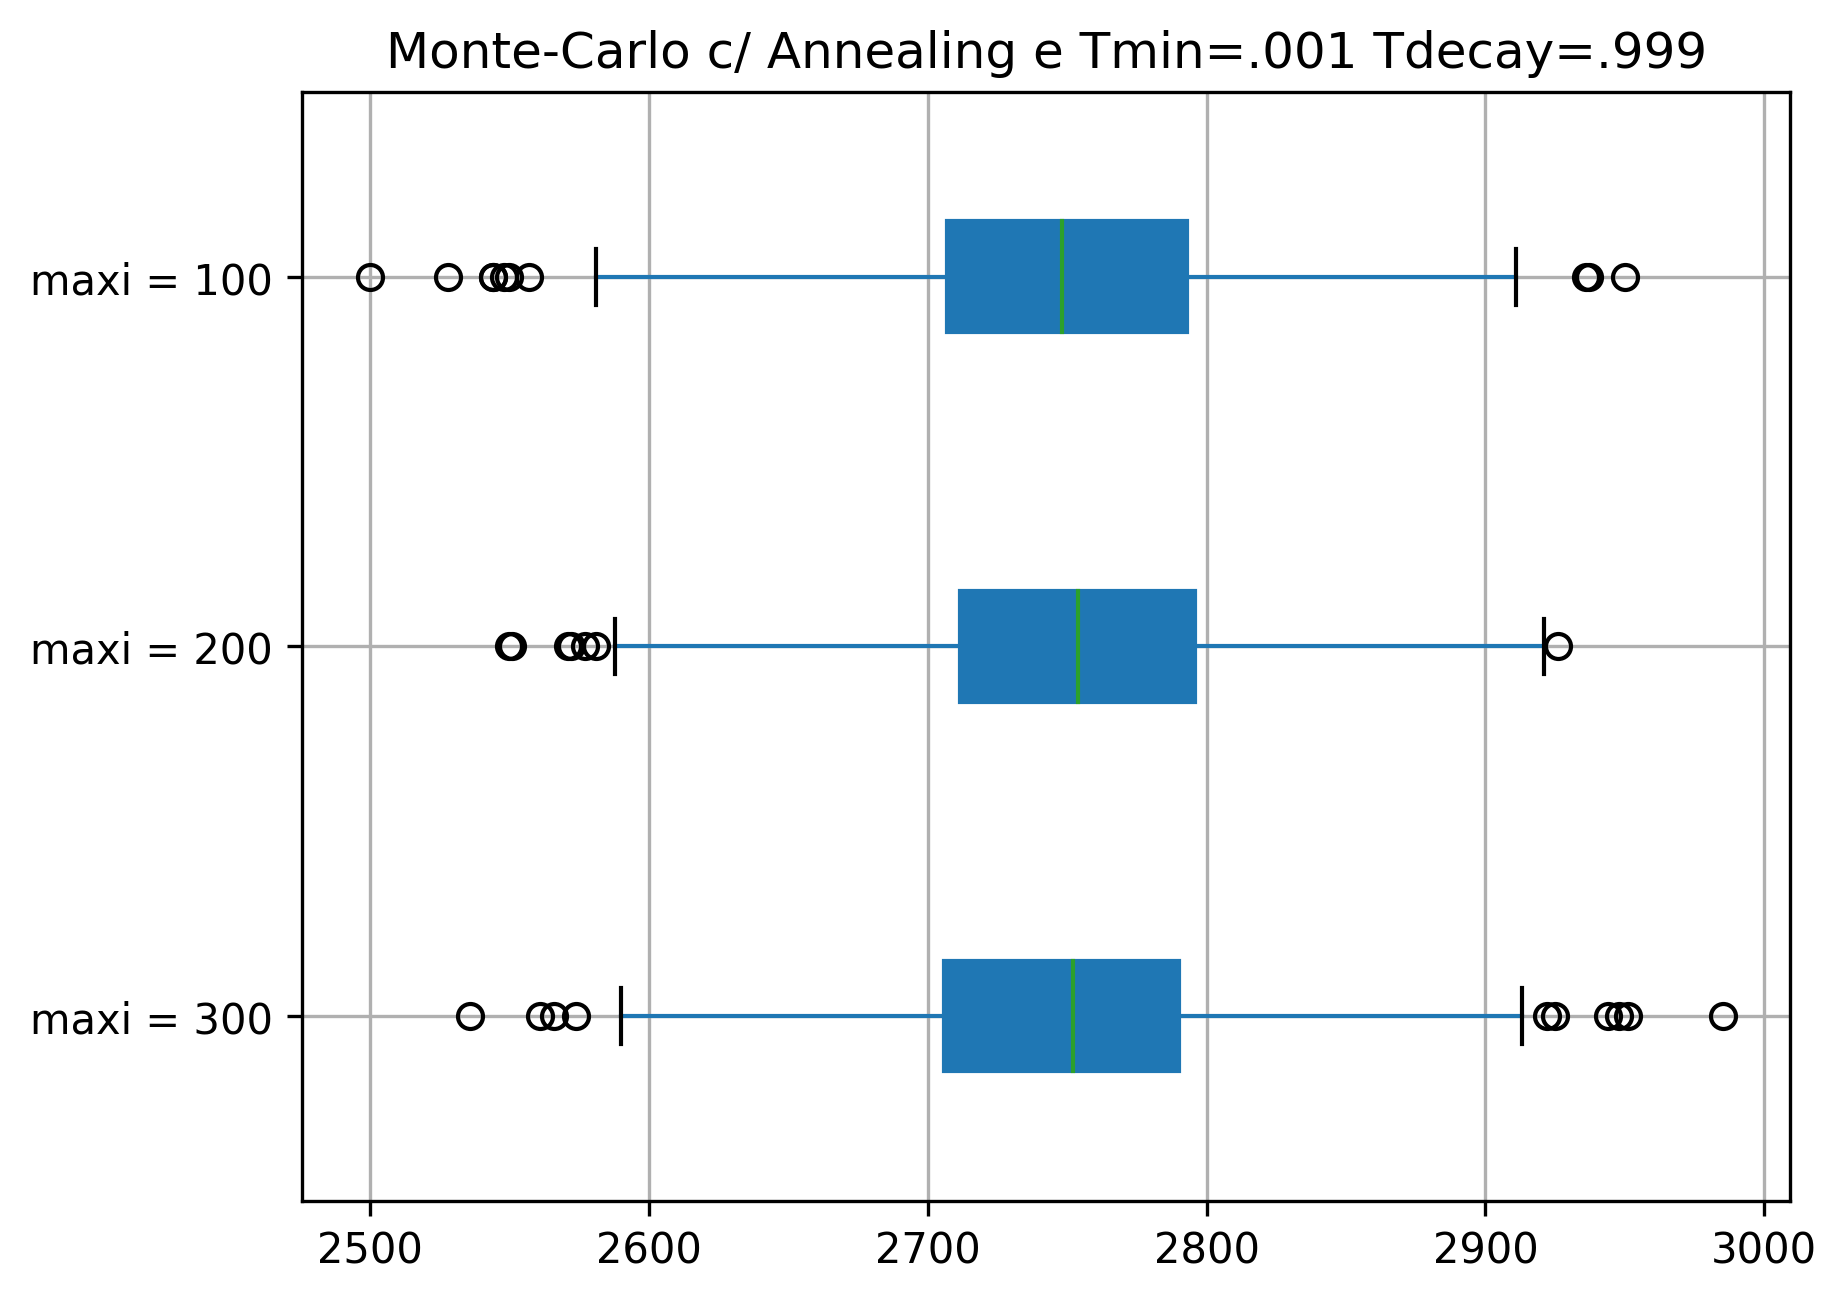
\includegraphics[width=.95\linewidth]{images/graph_comp_maxi_sa.png}
\end{minipage}
    \caption{Comparação de diferentes valores para maxi em Monte-Carlo com e sem annealing}
\end{figure}

A variável maxi define o numero máximo de iterações que podem ser realizadas sem
ocorrer alterações no custo da distribuição pelas salas.

No caso do Monte-Carlo sem Annealing, aumentar o maxi permite aumentar o número
de ciclos em que se procura por uma solução melhor do que a que se tem
atualmente. Por isso, quanto maior o maxi melhor os resultados obtidos.

Por outro lado, no caso de Monte-Carlo com Annealing, como é possível fazer
trocas mesmo que não seja para melhorar o custo, o caso de paragem do algoritmo
é quase sempre quando a temperatura atinge o tmin, fazendo com que o maxi não
tenha grande impacto no resultado obtido. Desta forma, todos os testes foram
efetuados com o valor de maxi a 100.

\begin{figure}[h]
\centering
\begin{minipage}{.5\textwidth}
  \centering
  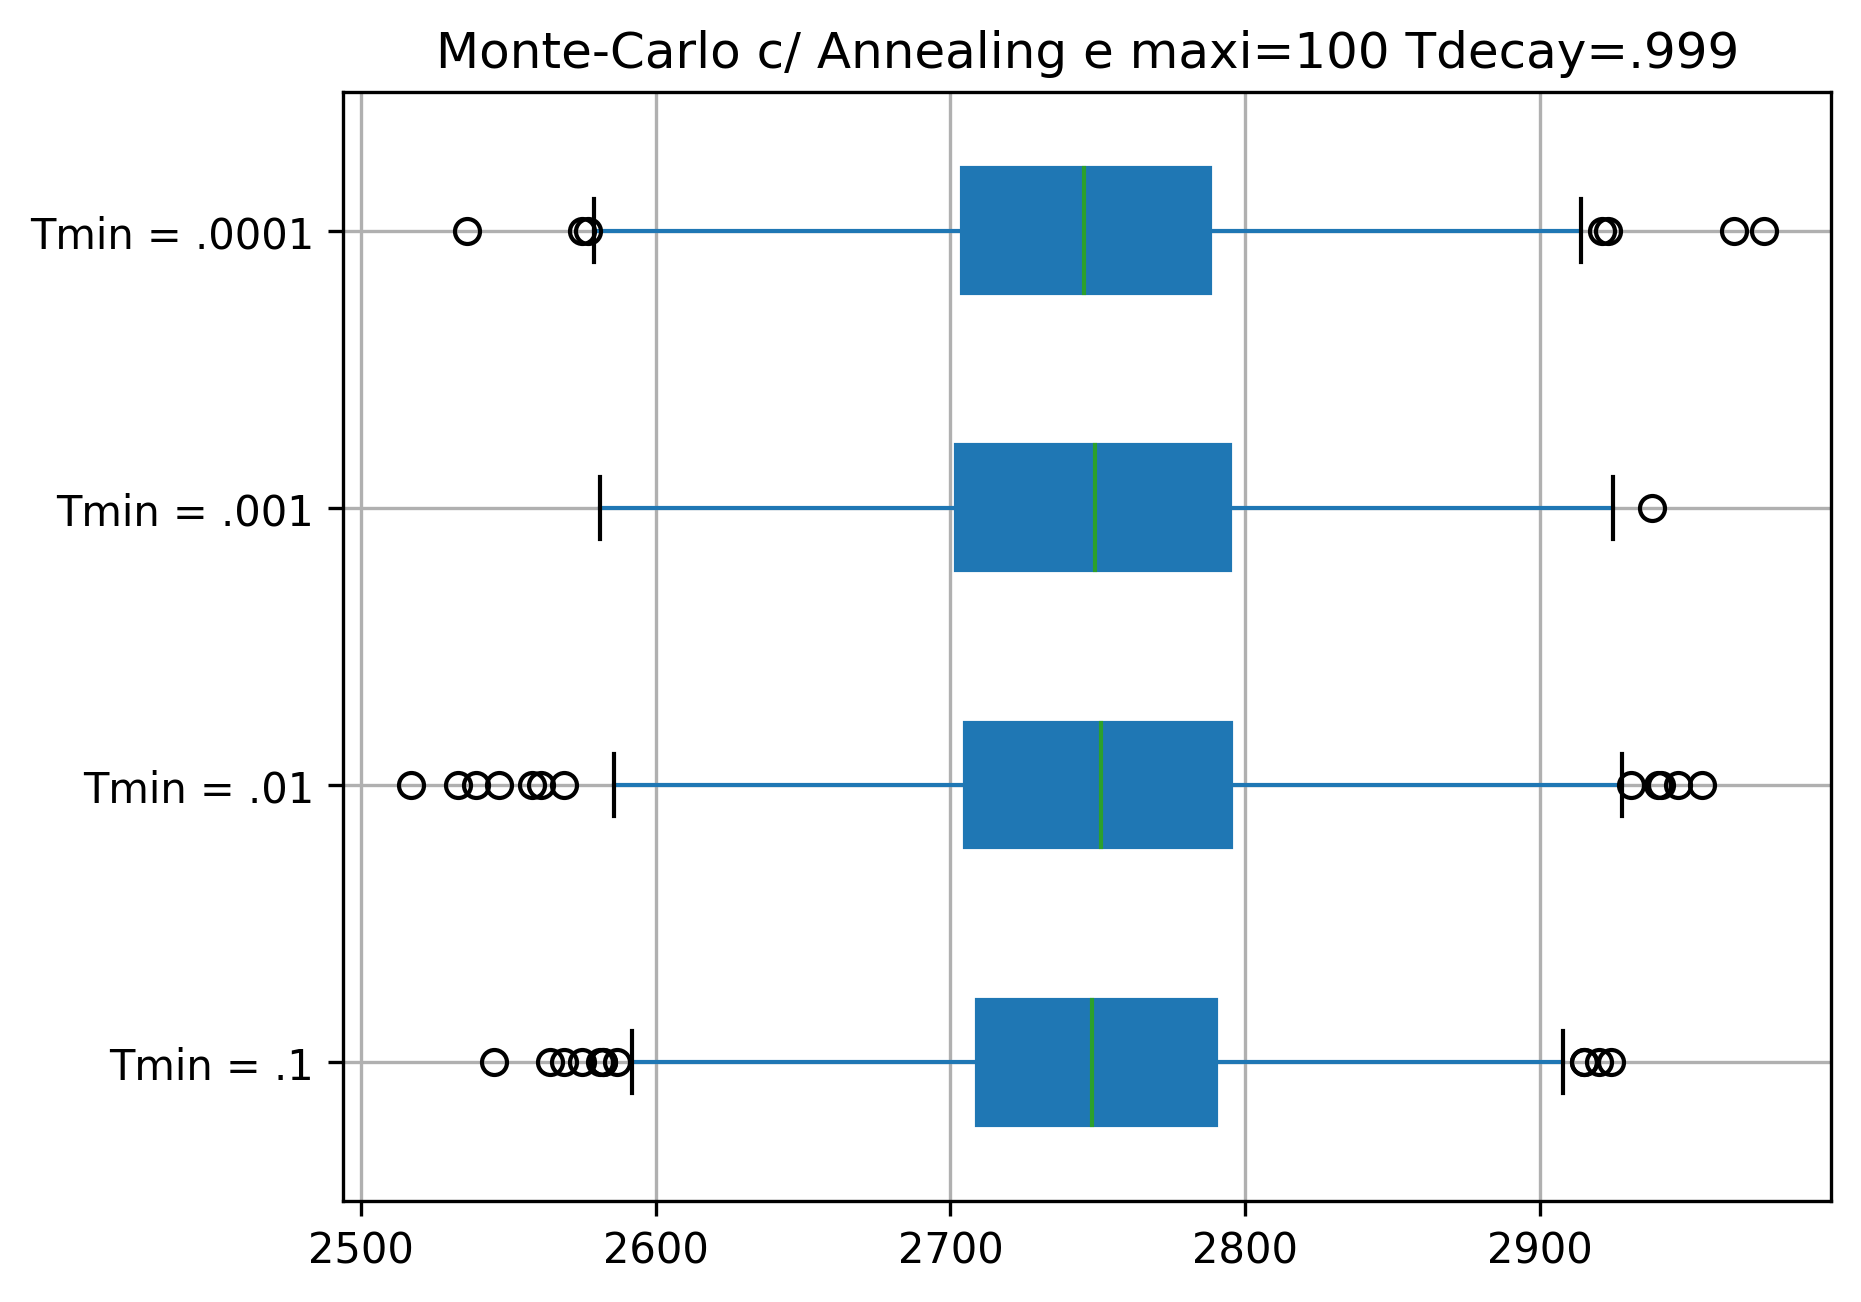
\includegraphics[width=.95\linewidth]{images/graph_comp_tmin_sa.png}
\end{minipage}%
\begin{minipage}{.5\textwidth}
  \centering
  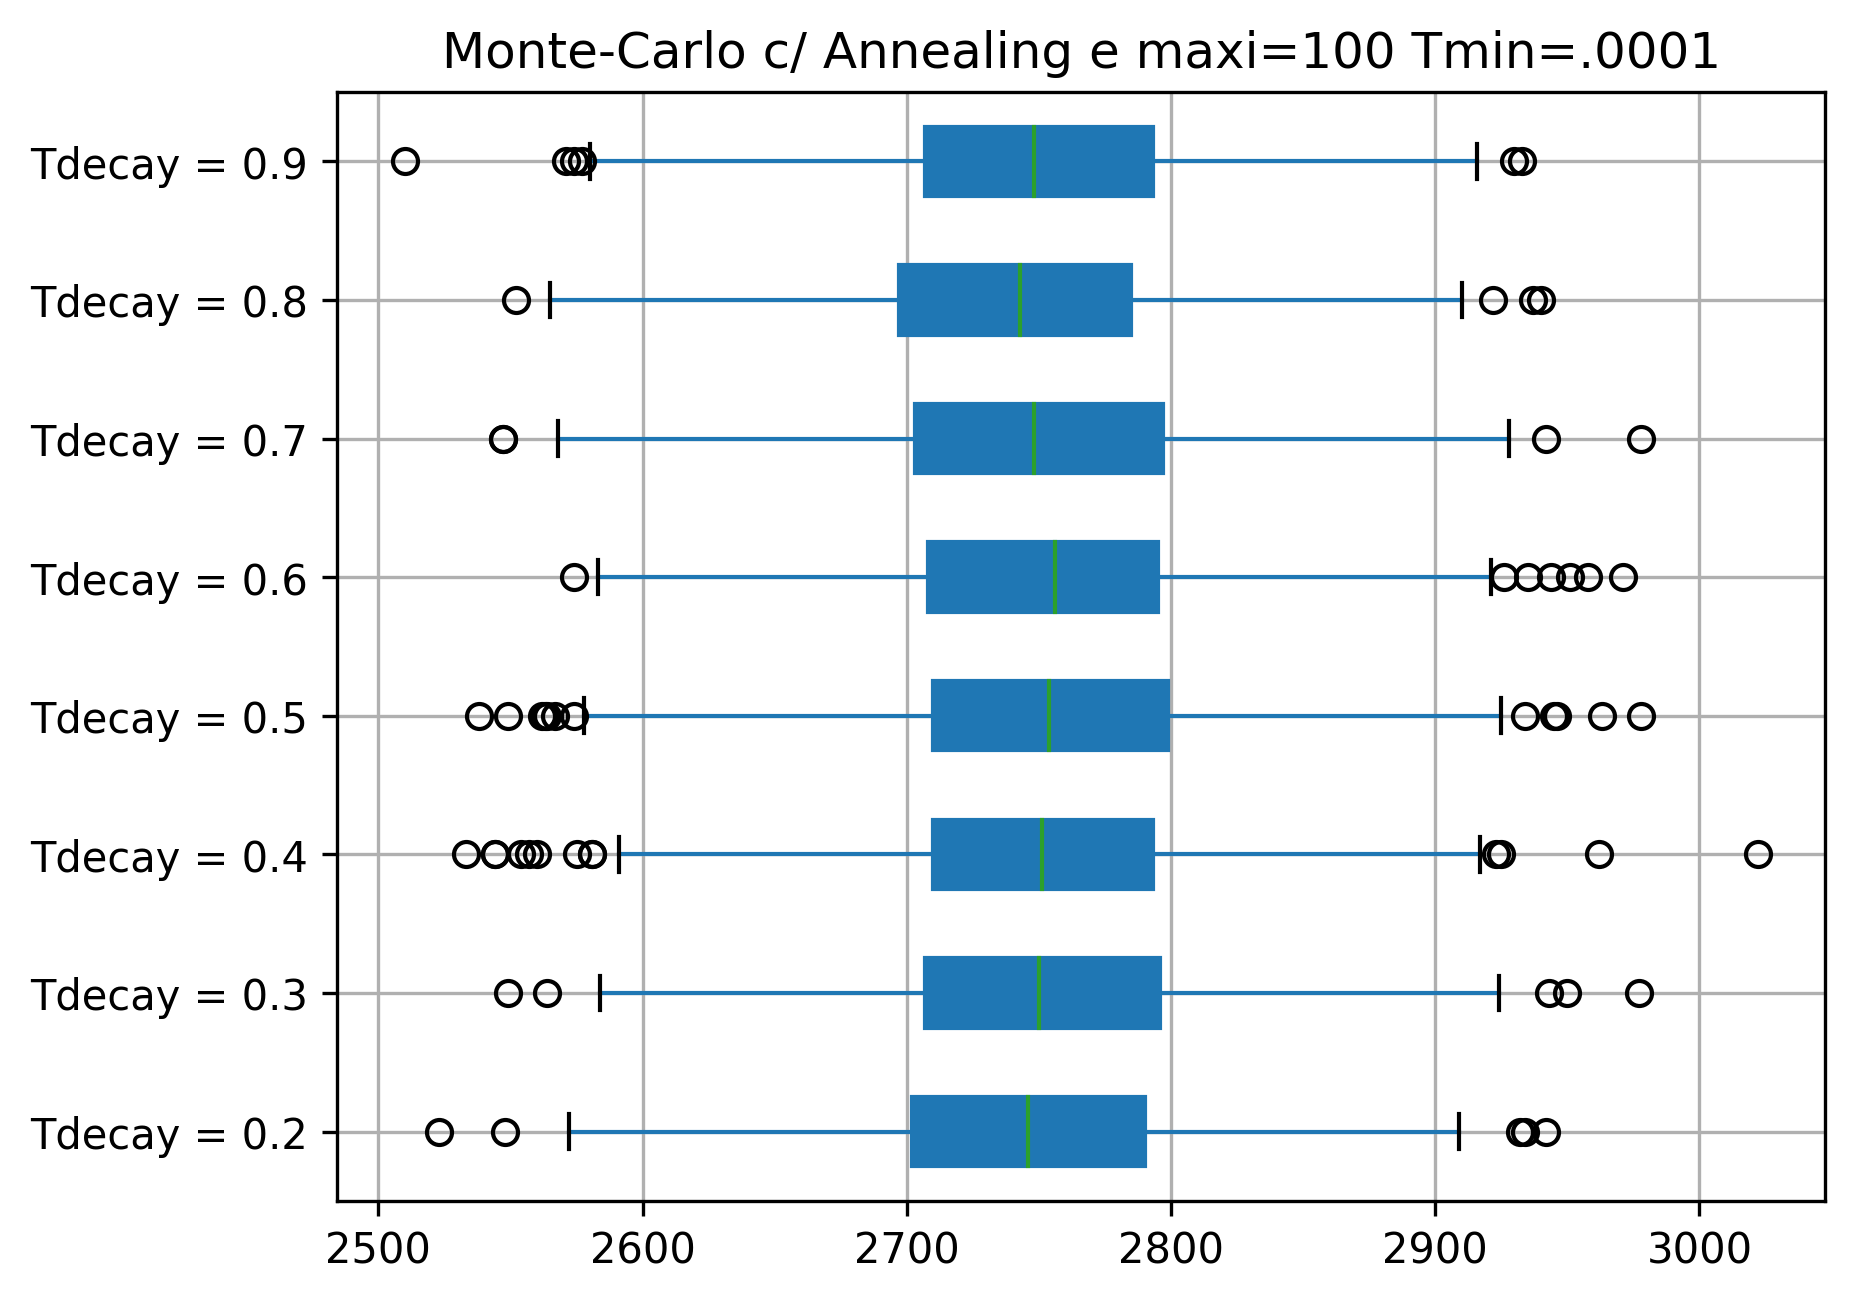
\includegraphics[width=.95\linewidth]{images/graph_comp_tdecay_sa.png}
\end{minipage}
    \caption{Comparação de diferentes valores para Tmin e Tdecay em Monte-Carlo com annealing}
\end{figure}

\pagebreak
Como podemos ver, embora sejam pequenas variações, quanto
menor o Tmin, mais concentrados os resultados obtidos, graças ao maior número de
iterações efetuadas. Esta diminuição leva também a que tanto os quartis como a
mediana apresentam valores mais baixos, o que corresponde, regra geral, à obtenção de
melhores resultados.

Com a variação do Tdecay, não há nenhuma tendência explicita definida, pois com
a diminuição deste são efetuadas menos iterações, mas ao mesmo tempo, são
efetuadas menos trocas que possam contribuir para a obtenção de resultados
piores. Por outro lado, ao aumentar o Tdecay, temos mais iterações do
algoritmo, mas podendo este ter mais trocas que contribuam para a obtenção de um
custo superior.

\pagebreak
\begin{figure}[h]
    \centering
        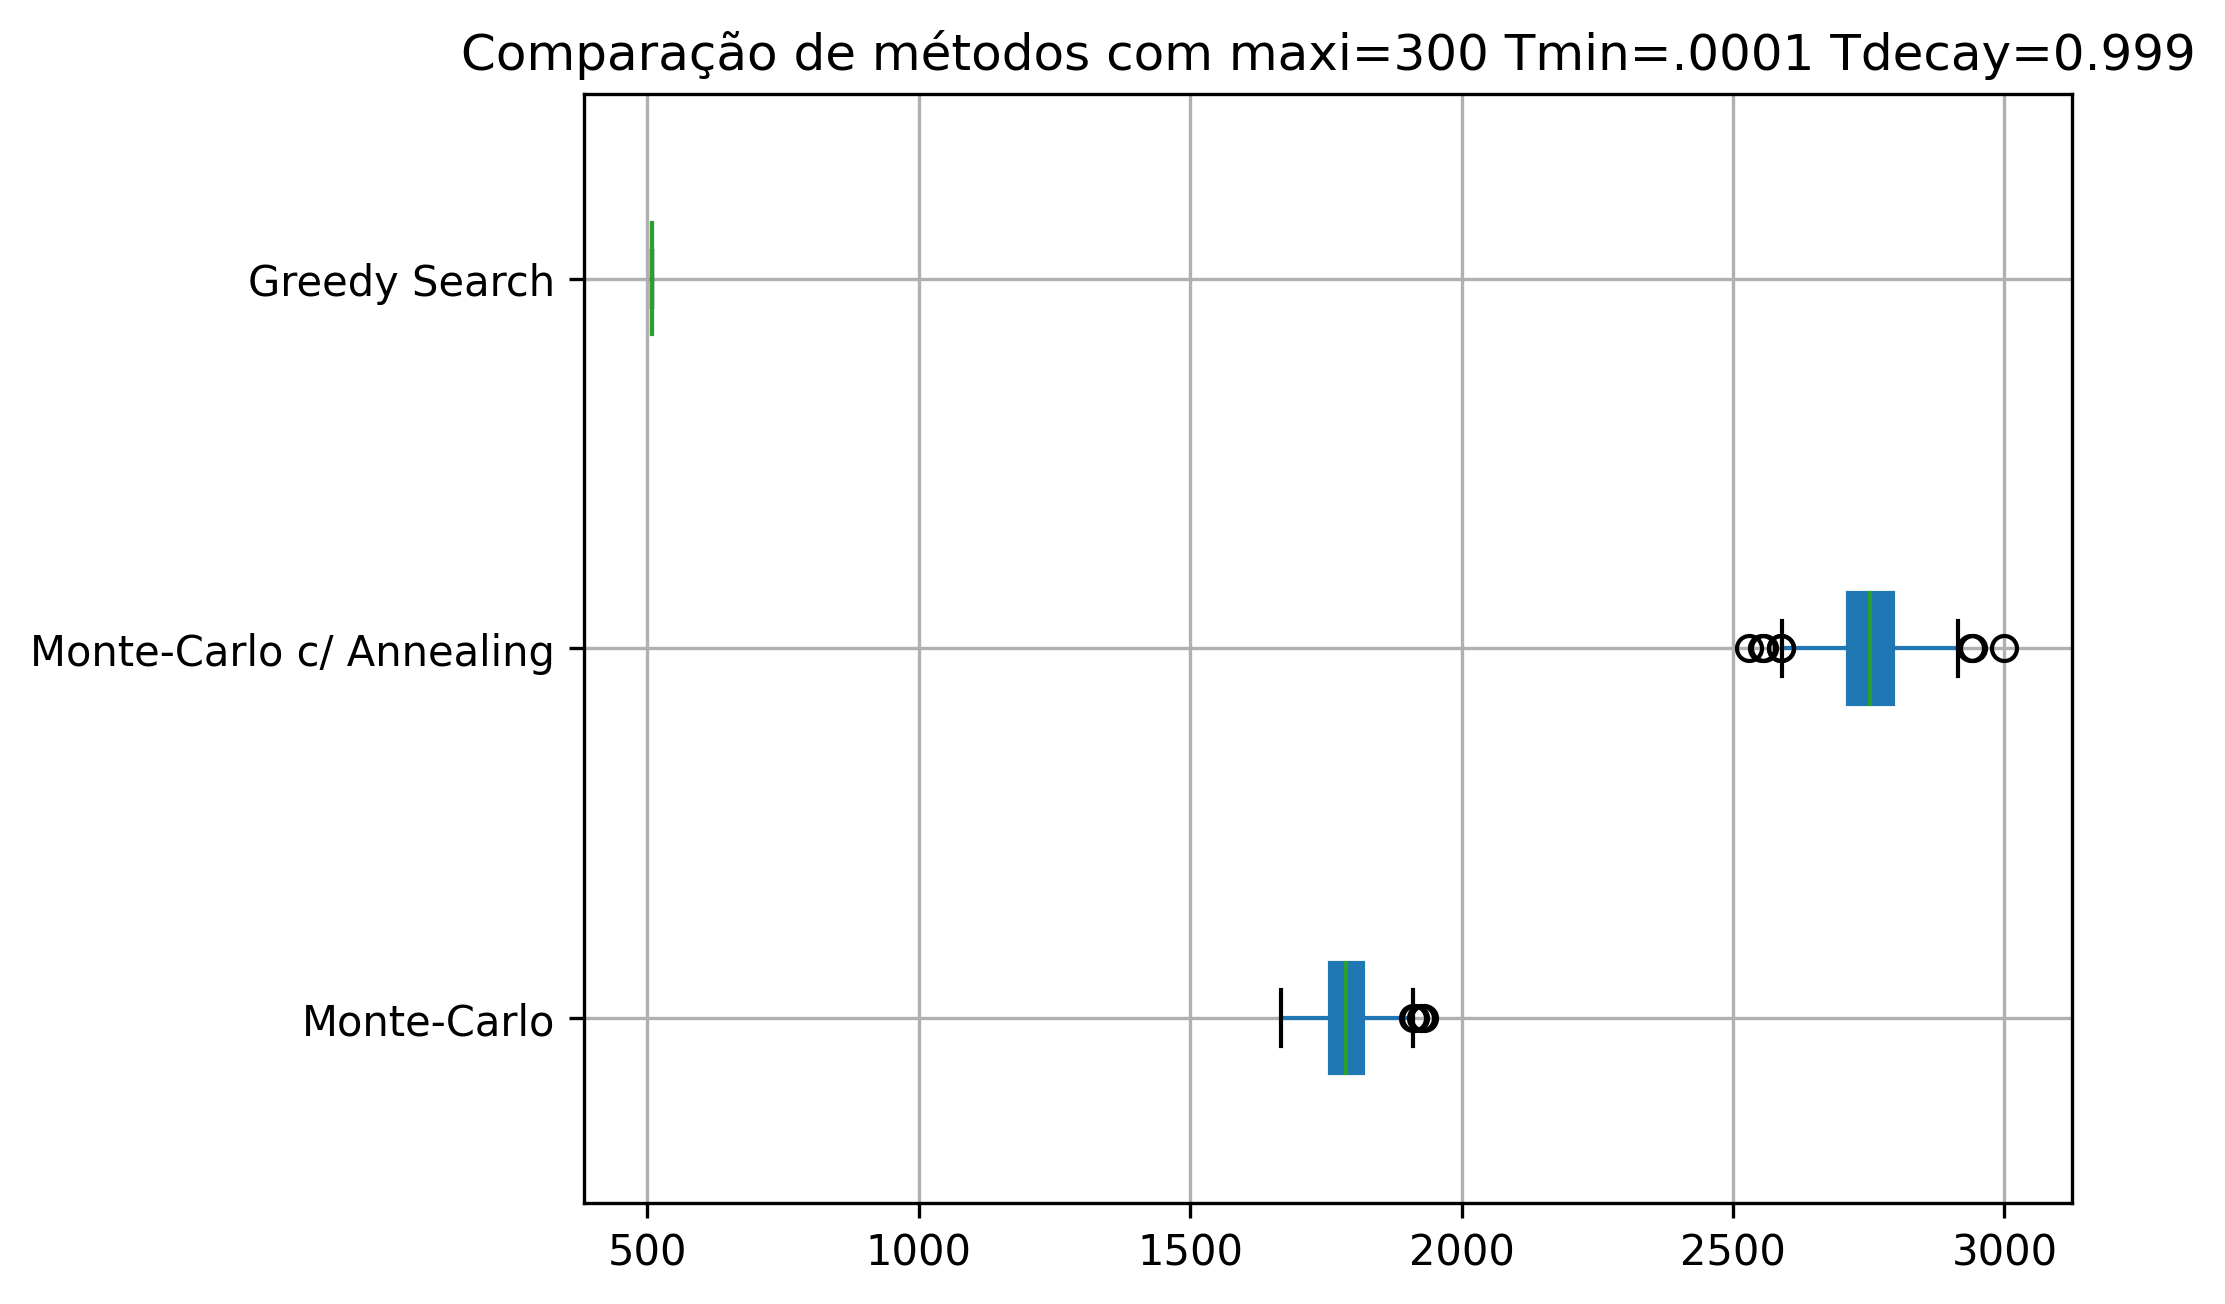
\includegraphics[width=\textwidth]{images/graph_comp_all_algorithms.png}
        \caption{Comparação de todos os métodos desenvolvidos}
\end{figure}

Comparando o algoritmo que utilizada Monte-Carlo com o que utiliza também
Annealing, podemos ver que o que utiliza apenas Monte-Carlo produz resultados
substancialmente melhores que o que também utiliza Annealing, visto que este
ultimo realiza trocas desnecessárias e prejudiciais ao bom resultado do
algoritmo.

Comparando os anteriores com a pesquisa Greedy, vemos que a pesquisa Greedy
produz o melhor resultado comparado com todos os anteriores, pois como o
intervalo de valores a escolher é muito restrito quando comparado com o número
de pessoas que utlizamos para testar, faz com que exista sempre um valor muito
pequeno para a relação entre duas pessoas, o que é extremamente benéfico para o
funcionamento deste algoritmo, levando quase sempre a uma solução otima ou muito
perto desta.

\end{document}
